%%%%%%%%%%%%%%%%%%%%%%%%%%%%%%%%%%%%%%%%%
% a0poster Landscape Poster
% LaTeX Template
% Version 1.0 (22/06/13)
%
% The a0poster class was created by:
% Gerlinde Kettl and Matthias Weiser (tex@kettl.de)
% 
% This template has been downloaded from:
% http://www.LaTeXTemplates.com
%
% License:
% CC BY-NC-SA 3.0 (http://creativecommons.org/licenses/by-nc-sa/3.0/)
%
%%%%%%%%%%%%%%%%%%%%%%%%%%%%%%%%%%%%%%%%%

%----------------------------------------------------------------------------------------
%	PACKAGES AND OTHER DOCUMENT CONFIGURATIONS
%----------------------------------------------------------------------------------------

%\documentclass[a4,portrait,25pt]{sciposter}
%\documentclass{article}
\documentclass[20pt]{extreport}

%\usepackage{multicol,caption} % This is so we can have multiple columns of text side-by-side
%\columnsep=100pt % This is the amount of white space between the columns in the poster
%\columnseprule=3pt % This is the thickness of the black line between the columns in the poster
\usepackage[margin=0.3in]{geometry}
\usepackage[svgnames]{xcolor} % Specify colors by their 'svgnames', for a full list of all colors available see here: http://www.latextemplates.com/svgnames-colors

%\usepackage{times} % Use the times font
%\usepackage{palatino} % Uncomment to use the Palatino font

\usepackage{graphicx} % Required for including images
\graphicspath{{figures/}} % Location of the graphics files
\usepackage{booktabs} % Top and bottom rules for table
\usepackage[font=small,labelfont=bf]{caption} % Required for specifying captions to tables and figures
\usepackage{amsfonts, amsmath, amsthm, amssymb} % For math fonts, symbols and environments
%\usepackage{wrapfig} % Allows wrapping text around tables and figures


\usepackage{listings}
\usepackage{amsfonts}
\usepackage{tabularx}
\usepackage{enumitem}

\usepackage{tikz}
\usepackage{graphicx}
\usepackage{subfig}


\usepackage{lipsum}

%\usepackage[boxruled]{algorithm2e}
%\usepackage{algorithm}% http://ctan.org/pkg/algorithm
\usepackage[noend]{algpseudocode}% http://ctan.org/pkg/algorithmicx
\usepackage{algorithm}% http://ctan.org/pkg/algorithms

\newtheorem{Def}{Definition}
\newtheorem{Theorem}{Theorem}

\usetikzlibrary{arrows,positioning} 



\usetikzlibrary{arrows,positioning} 
\pgfarrowsdeclarecombine{ring}{ring}{}{}{o}{o}

\DeclareMathOperator{\ringarrow}{\raisebox{0.5ex}{\tikz[baseline]{\draw[ring->](0,0)--(2em,0);}}}

\tikzset{
    %Define standard arrow tip
    >=stealth',
    %Define style for boxes
    punkt/.style={
           circle,
           rounded corners,
           draw=black, thick,
           minimum width=.5em,
           minimum height=.5em,
           font=\small,
           text centered},
    punktrect/.style={
    rectangle, 
    rounded corners, 
    % fill=black!10,
    draw=black, thick,
    minimum height=1em, 
    text centered},
    % Define arrow style
    pil/.style={
           o->,
           thick,
           shorten <=2pt,
           shorten >=2pt,}
}

\title{Causal Inference in Machine Learning: A Review}
\author{Finnian Lattimore\\ Australian National University\\finnlattimore@gmail.com\\\textbf{Apologies,}\\ \textbf{the poster is in Air Canada's lost baggage area} }

\begin{document}
\def\ci{\perp\!\!\!\perp}
\maketitle
%----------------------------------------------------------------------------------------
%	POSTER HEADER 
%----------------------------------------------------------------------------------------

% The header is divided into three boxes:
% The first is 55% wide and houses the title, subtitle, names and university/organization
% The second is 25% wide and houses contact information
% The third is 19% wide and houses a logo for your university/organization or a photo of you
% The widths of these boxes can be easily edited to accommodate your content as you see fit
%\begin{minipage}[t]{0.15\linewidth}%
%\centering
%
\includegraphics[height=12cm]{nicta_logo2.jpg} % Logo or a photo of you, adjust its dimensions here
%\end{minipage}
%\begin{minipage}[b]{0.65\linewidth}
%\centering
%\resizebox{\linewidth}{!}{\veryHuge \color{NavyBlue} \textbf{Causal Inference in Machine Learning: %A review}}
% \color{Black}\\ 

%\huge \textbf{Finnian Lattimore}\\ % Author(s)
%\huge Australian National University\\ % University/organization
%finnlattimore@gmail.com

%\end{minipage}
%\begin{minipage}[t]{0.15\linewidth}
%\centering
%
\includegraphics[height=12cm]{anu-logo-notext}
%\end{minipage}


%----------------------------------------------------------------------------------------

%\begin{multicols}{2} % This is how many columns your poster will be broken into, a poster with many figures may benefit from less columns whereas a text-heavy poster benefits from more


%----------------------------------------------------------------------------------------
%	INTRODUCTION
%----------------------------------------------------------------------------------------

%\color{DarkSlateGray} % DarkSlateGray color for the rest of the content

\section*{Introduction}

Would cutting salt intake reduce heart attack risk? Would upping the minimum wage increase unemployment? Causal problems differ from the traditional machine learning setting in that they require us to predict the consequences of an intervention, which may change the properties of the distribution from which our data is sampled. Without experimentally testing the intervention or making assumptions to constrain its effect, such inference is impossible. There are many important questions where direct experimentation is expensive, unethical or impossible. Recent research on causality has clarified what assumptions allow causality to be determined and has demonstrated causal inference and discovery is possible with some very general assumptions.   

\section*{Causal Frameworks}
\subsection*{Causal Directed Acyclic Graphs}
\begin{itemize}
\item A causal DAG is a Bayesian network where $A \rightarrow B$ is defined to mean $A$ causes $B$.
\item Variables are independent of their non-effects given their direct causes (Causal Markov Property)
\item An intervention that sets a subset of variables $\boldsymbol{X}$ to $\boldsymbol{x}$, denoted $do(\boldsymbol{X} = \boldsymbol{x})$, has a simple graphical representation in a causal DAG, $G$. All links entering intervened on variables, $\boldsymbol{X}$, are deleted, resulting in the mutilated network $G_{\overline{\boldsymbol{X}}}$ (figure \ref{fig:intervention}). Thus, a causal DAG represents the set of all possible interventional distributions over its variables.
\end{itemize}

\begin{figure}
\caption{Intervention in a causal DAG}
\label{fig:intervention}
\centering
{\resizebox{\columnwidth}{!}{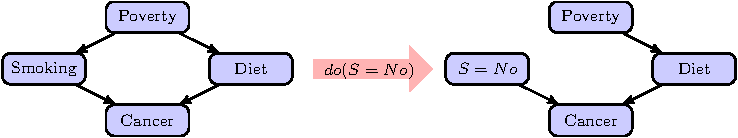
\includegraphics{intervention_figure-crop}}}
\end{figure}

\subsection*{(Causal) Structural Equation Models (SEMs)}
\begin{itemize}
\item Represent each variable as a deterministic function of its direct causes and a noise term, where the noise terms are mutually independent.

\item If the set of equations does not create a cycle then the Causal Markov Property holds and the SEM is a causal DAG, (but not visa-versa - SEMs can encode more information).
\end{itemize}


\subsection*{Counterfactuals}
\begin{itemize}
\item Counterfactuals are statements about what would happen under alternate realities where some specified thing differs. For example, consider people taking a medical drug:

For an individual, $i$, let: $\begin{cases}y^{0}_{i} =& \text{outcome if $x_{i}=0$ (not treated)} \\ y^{1}_{i} =& \text{outcome if $x_{i}=1$ (treated)}
\end{cases}$ 

\item We can define a random variable $Y^{1}$, where $P(Y^{1})$ is the distribution of outcome, $Y$, that would occur if everyone was treated. Similarly $P(Y^{0})$ is the distribution of outcome if no-one was treated. 
\item If   $(X \ci Y^{0}|\boldsymbol{Z})$ \&  $(X\ci Y^{1}|\boldsymbol{Z})$:  $\longleftarrow$ Ignoreability Assumption \\*
we can calculate counterfactual distributions from observed ones:
\begin{equation*}
P(Y^{1}|Z) = P(Y|X=1,Z) \text{ and } P(Y^{0}|Z) = P(Y|X=0,Z)
\end{equation*}

\item Distributions over counterfactual variables that correspond to interventions can be translated directly to the do notation $P(Y^{1}) = P(Y|do(X=1))$. However we can phrase queries with counterfactual variables that are not interventional. For example: \textit{what is the proability that Joe, who was not treated and died, would have recovered had he been treated?}. This query asks about the joint distribution of $P(Y^{0},Y^{1})$. 

\begin{center}
\begin{tabular}{c|c|c|c}
group & placebo & treatment & probability of group\\
\hline
1 & die & die & $\alpha=P(Y^{0}=0,Y^{1}=0)$\\
2 & die & recover & $\beta=P(Y^{0}=0,Y^{1}=1)$\\
3 & recover & die & $\gamma=P(Y^{0}=1,Y^{1}=0)$\\
4 & recover & recover & $\delta=P(Y^{0}=1,Y^{1}=1)$\\
\end{tabular}
\end{center}

\item Counterfactuals can be defined in terms of SEMs $Y^0 \sim f(X=0,\epsilon_Y)$ 
\item The ignorability assumption $(X \ci Y^{0}|\boldsymbol{Z})$ \&  $(X\ci Y^{1}|\boldsymbol{Z})$ is weaker than that implied by mutually independent errors in a SEM, $(X \ci Y^0,Y^1 | \boldsymbol{Z})$. The assumptions can be made equivalent by utilizing SEMs with a modified independence of errors assumption \cite{Richardson2013}. 

\end{itemize}



\section*{Causal Inference}

Consider the problem where the causal DAG is known, due to theory or prior knowledge, and we wish to infer the outcome of an intervention of the form $P(\boldsymbol{Y}|do(\boldsymbol{X}=\boldsymbol{x}))$ using observational data.

\begin{itemize}
\item If there are no latent variables, we can compute outcome of any intervention by simply multiply the factors in the mutliated network (figure \ref{fig:intervention}).
\end{itemize}



\subsection*{The Do Calculus}

The do-calculus consists of three rules, which result from d-separation in a causal DAG \cite{Pearl2000}. It is complete: a causal effect is non-parametrically identifiable if and only if the interventional query can be reduced to an observational one via these rules \cite{Shpitser2008}. 

\begin{figure}
\caption{d-separation allows us to read conditional independences off a DAG. If a set of variables $\boldsymbol{Z}$ d-separates $\boldsymbol{X}$ and $\boldsymbol{Y}$ in $G$ then ${(\boldsymbol{X} \ci \boldsymbol{Y}|\boldsymbol{Z})}$ in all distributions $P$ compatible with $G$. }
\label{fig:dsep}
\centering
{\resizebox{\columnwidth}{!}{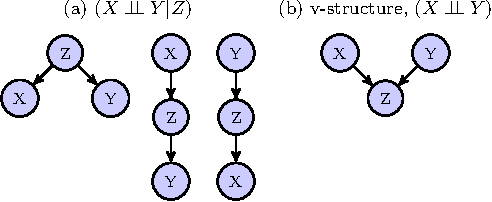
\includegraphics{dsepfigure-crop}}}
\end{figure}

\begin{center} 
\fbox{\begin{minipage}{0.9\textwidth}%
\textbf{The Three Rules}
\begin{enumerate}
\item A causal DAG remains a causal DAG after an intervention so d-separation still applies.
\begin{equation*}
\label{eq:Do1}
\begin{aligned}
& \text{if }  (\boldsymbol{Y} \ci  \boldsymbol{W}|\boldsymbol{X})  \text{ in } G_{\overline{\boldsymbol{X}}}  \\
& P(\boldsymbol{Y}|do(\boldsymbol{X}=\boldsymbol{x}),\boldsymbol{W}=\boldsymbol{w}) = P(\boldsymbol{Y}|do(\boldsymbol{X}=\boldsymbol{x})) 
\end{aligned}
\end{equation*}
\item If $\boldsymbol{Y}$ is independent of \textit{how} variables $\boldsymbol{X}$ take their values then the effect on $\boldsymbol{Y}$ of setting $\boldsymbol{X}$ to some value is equivalent to observing it take that value. If this rule is satisfied the corresponding ignoreability assumption in the counterfactual framework is satisfied.
\begin{equation*}
\label{eq:Do2}
\begin{aligned}
& \text{if } (\boldsymbol{Y} \ci  \boldsymbol{\hat{X}}|\boldsymbol{X},\boldsymbol{Z})  \text{ in } G^{\dagger}\\
& P(\boldsymbol{Y}|do(\boldsymbol{X}=\boldsymbol{x}),\boldsymbol{Z}) = P(\boldsymbol{Y}|\boldsymbol{X}=\boldsymbol{x},\boldsymbol{Z})
\end{aligned}
\end{equation*}
\item If there is no direct causal path from $\boldsymbol{X}$ to $\boldsymbol{Y}$ then intervention on $\boldsymbol{X}$ does not change the distribution of $\boldsymbol{Y}$.
\begin{equation*}
\label{eq:Do2}
\begin{aligned}
&\text{if }  (\boldsymbol{Y} \ci  \boldsymbol{\hat{X}}|\boldsymbol{Z})  \text{ in } G^{\dagger}\\
& P(\boldsymbol{Y}|do(\boldsymbol{X}=\boldsymbol{x}),\boldsymbol{Z}) = P(\boldsymbol{Y}|\boldsymbol{Z})
\end{aligned}
\end{equation*}
\end{enumerate}
\footnotesize (For readability, this is a simplified version of the do-calculus that covers interventions on a single variable or cases where it is sufficient for identifiability to consider intervention on all variables together. The fully general version is only slightly more complex see \cite{Pearl2000})
\normalsize
\end{minipage}}
\end{center}

%\columnbreak
\section*{Causal Discovery}

Causal discovery attempts to infer causal structure from data based on more general assumptions. 

\subsection*{Indepdendence Based Methods}
\subsubsection*{Without Latent Variables}
\begin{enumerate}
\item We assume our distribution $P$ was generated by some (unknown) causal DAG over our observed variables (\emph{causal sufficiency}) 
\item We assume that all the conditional independences in $P$ are implied by d-separation in the true causal network (\emph{faithfulness}) 
\item Finding the causal structure equates to finding perfect maps for $P$
\end{enumerate}

\begin{algorithm}
\caption{SGS or IC Algorithm \cite{Sprites,Pearl2000}. \label{alg:spect}}
\textbf{Input:} A Distribution $P$ over variables $\boldsymbol{V}$

\textbf{Output:} A partially directed network representing the Markov equivalence class for the generating causal model.
\begin{enumerate}
\item Create a complete undirected graph over $V$. For all pairs of variables $(a,b) \in V$ search for a set $S_{ab}$ s.t $a \ci b|S_{ab}$. If such a set exists, delete the link $a-b$
\item For all pairs of unlinked-nodes $(\alpha, \beta)$ with a common neighbour $c$, if $c \notin S_{\alpha \beta}$ direct links towards $c$.
\item Recursively direct any remaining links for which there is only one orientation that does not create a cycle or any additional v-structures ( $\bullet \rightarrow \bullet \leftarrow \bullet$). 
\end{enumerate}
\end{algorithm}

\begin{figure}
\caption{The SGS Algorithm}
\label{fig:SGS}
\centering
{\resizebox{0.55\columnwidth}{!}{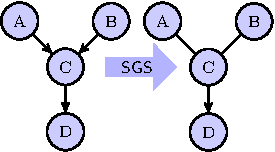
\includegraphics{SGS_figure-crop}}}
\end{figure}

\begin{itemize}
\item The SGS algorithm is infeasible in practise due to the exponential number of (high order) conditional independence tests it requires. 
\item 
The PC algorithm \cite{Sprites} modifies the SGS algorithm to exploit any sparsity in the true network, leading to much better average case performance.
\end{itemize}

\subsubsection*{With Latent Variables}
\begin{itemize}
\item For every latent structure there is a dependency equivalent structure in which every latent variable is a root node with exactly two children \cite{Verma1993}. This key to the FCI algorithm \cite{Sprites}, which generalizes the PC algorithm to handle latent and selection variables. 

\item The FCI algorithm returns an equivalence class of Maximal Ancestral Graphs (a generalization of DAGs) since DAGs are not closed under marginalization (figure \ref{fig:FCI}b).
\end{itemize}


\newcommand{\imsize}{.70\columnwidth}

\begin{figure}
\caption{The FCI Algorithm}
\label{fig:FCI}
\centering
{\resizebox{\columnwidth}{!}{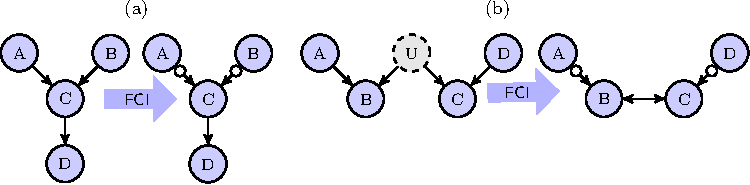
\includegraphics{FCI_figure-crop}}}
\end{figure}

\begin{itemize}
\item The FCI algorithm discovers all aspects of causal structure identifiable from conditional independence relations \cite{Zhang2008}.
\item It can be made to require a worst case polynomial (rather than exponential) number of conditional independence tests for sparse graphs \cite{Claassen2013}. 
\item Implementations of both the PC and FCI algorithm are available in the R package pcalg \cite{Kalisch2012}
\end{itemize}


\subsection*{Beyond independence}
Independence based methods have the advantage that they require only very general, non-parametric, assumptions. However they cannot distinguish between causal graphs with equivalent dependency structure; for example, between $X \rightarrow Y$ and $X \leftarrow Y$.


\begin{figure}
\centering
\caption{Figure from {\cite{Hoyer2009}}. Additive noise models, $Y = f(X)+\epsilon$, are identifiable for most combinations of $f$ and $P(\epsilon)$ but not in linear-gaussian case}
{\resizebox{\imsize}{!}{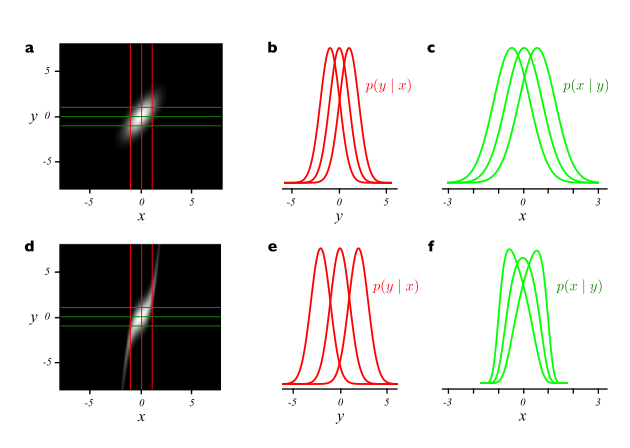
\includegraphics{Hoyer1}}}
\end{figure}

\begin{figure}
\centering
\caption{Figure from {\cite{Daniusis2010}}. The causal direction can be identifiable even where the relationship between $X$ and $Y$ is deterministic and invertible. Let $Y = f(X) \Leftrightarrow X = g(Y)$. For most input distributions, $p_{X}(x)$, the distribution $p_{Y}(y)$ will be higher where $f'$ is small and a larger region of $X$ maps to similar values of $Y$. If $X$ causes $Y$ (but not if $Y$ causes $X$) we would expect $f$ and $p_{X}(x)$ to be independent and $p_{Y}(y)$ should be correlated with $f'$.} 

{\resizebox{\imsize}{!}{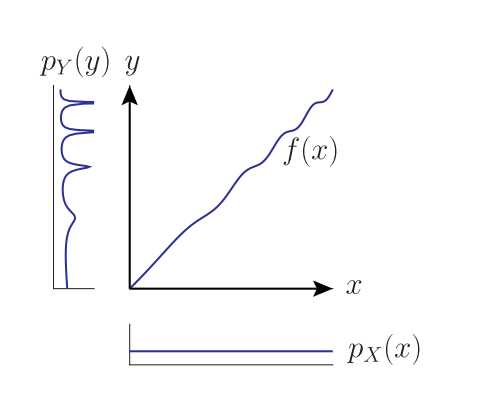
\includegraphics{Daniusis1}}}
\end{figure}

\begin{figure}
\centering
\caption{Figure from {\cite{Scholkopf2012}}. The idea of independence of mechanism and input can be generalized to the non-deterministic setting. If $X \rightarrow Y$ then $P(X)$ and $P(Y|X)$ should be independent, but $P(Y)$ and $P(X|Y)$ are not. Therefore, semi-supervised learning should yield no benefit when trying to learn in the causal direction, (estimating $P(Y|X)$) but could help when learning in the anti-causal direction.}
{\resizebox{\imsize}{!}{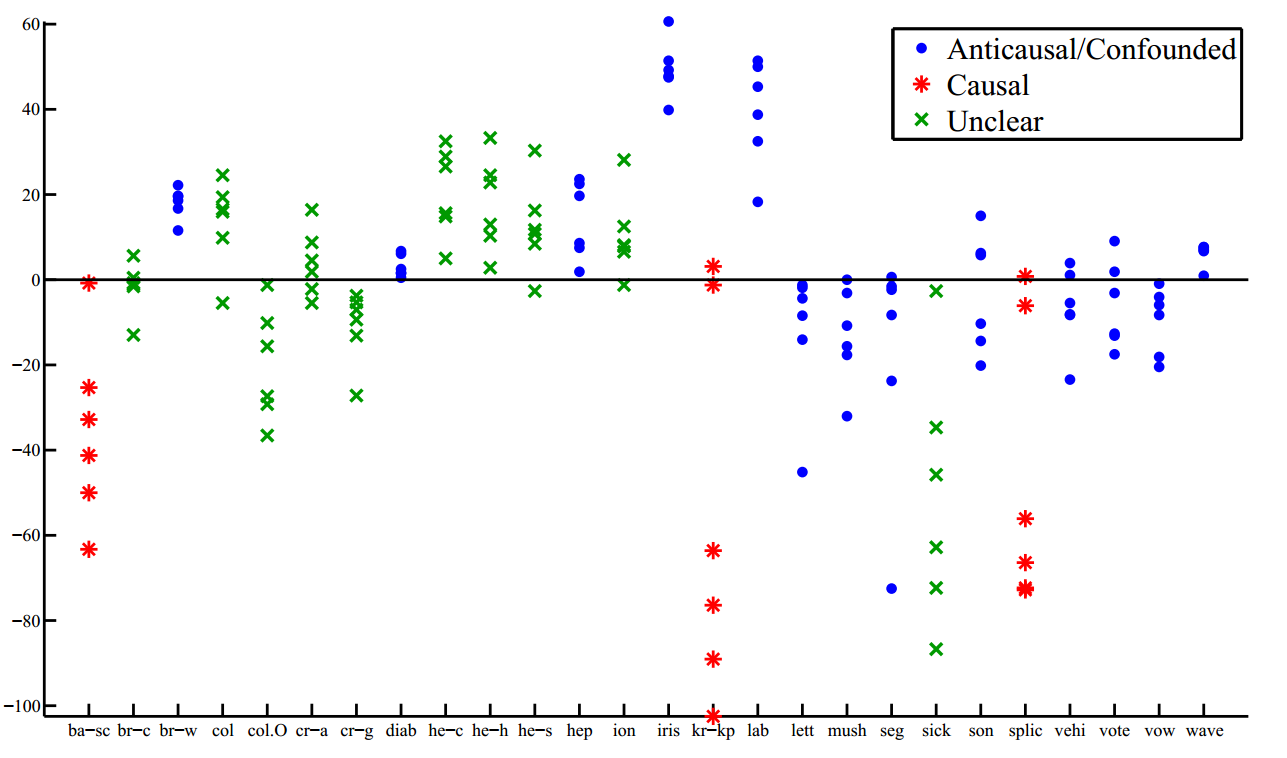
\includegraphics{Janzig61}}}
\end{figure}

\subsubsection*{Learning what causality looks like {\cite{LopezPaz2014}}}

Suppose we had $M$ different causal pairs data sets. 

\begin{equation*}
D= \{\{x_{j},y_{j}\}_{j=1}^{N_{i}},l_{i}\}_{i=1}^{M}
\end{equation*}

where $l_{i}$ is a binary label that indicates if $X \rightarrow Y$ or $Y \rightarrow X$ in dataset $i$.

\begin{itemize}
\item Kernel mean embedding allows us to take a distribution $P$ and transform it to a point in some Hilbert space.
\item We expect there to be differences in the relationships between $P(X)$, $P(Y)$ and $P(Y|X)$ for $X \rightarrow Y$ and $Y \rightarrow X$
\end{itemize}
 
\begin{algorithm}
\caption{\label{alg:causallearn}}
\begin{enumerate}
\item Let $\mu$ be a kernel mean embedding that maps a distribution $P$ into some Hilbert space.
\item For each data set $i={1...M}$, construct a feature vector that approximates ${\mu(P(X)), \mu(P(Y)),\mu(P(X,Y)) }$
\item Apply a standard classification algorithm to learn if $X\rightarrow Y$ or $Y \rightarrow X$
\end{enumerate}
\end{algorithm}
\subsubsection*{With more than two variables}
\begin{itemize}
\item If you can come up with a condition, on the triple $(P(Y), P(\epsilon), f)$, that guarantees identifiability for the bi-variate SEM $Y = f(X) + \epsilon$, you can extend that result to get the conditions under which the multivariate case is identifiable \cite{Peters2014}.

\end{itemize}
%----------------------------------------------------------------------------------------
%	CONCLUSIONS
%----------------------------------------------------------------------------------------

\color{SaddleBrown} % SaddleBrown color for the conclusions to make them stand out




\color{DarkSlateGray} % Set the color back to DarkSlateGray for the rest of the content


 %----------------------------------------------------------------------------------------
%	REFERENCES
%----------------------------------------------------------------------------------------

\bibliographystyle{plain} % Plain referencing style
\bibliography{library} % Use the example bibliography file sample.bib


%\end{multicols}
\end{document}


We present a survey of recent results, focusing on the problems of inferring causal effects from observational data and causal discovery.


  \begin{minipage}{\columnwidth}
    \makeatletter
    \newcommand{\@captype}{figure}
    \makeatother
    \centering
    \subfloat[Market revenue]{%
    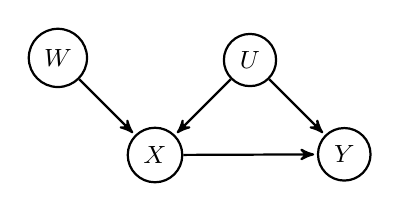
\begin{tikzpicture}[->,>=stealth',shorten >=1pt,auto,node distance=1cm,
  thick,main node/.style={punkt}]

 %nodes
\node[main node](1){$U$};
\node[main node, below left=of 1](2){$X$};
\node[main node, below right=of 1](3){$Y$};
\node[main node, above left=of 2](4){$W$};


 \path[every node/.style={font=\sffamily\small}]
    (1) edge node {} (2)
    	edge node {} (3)
    (2) edge node {} (3)
    (4) edge node {} (2);
	
\end{tikzpicture} 
      
      \label{fig:evaluation:revenue}%
    }\qquad%
    \subfloat[Average price]{%
    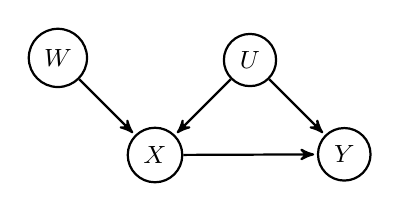
\begin{tikzpicture}[->,>=stealth',shorten >=1pt,auto,node distance=1cm,
  thick,main node/.style={punkt}]

 %nodes
\node[main node](1){$U$};
\node[main node, below left=of 1](2){$X$};
\node[main node, below right=of 1](3){$Y$};
\node[main node, above left=of 2](4){$W$};


 \path[every node/.style={font=\sffamily\small}]
    (1) edge node {} (2)
    	edge node {} (3)
    (2) edge node {} (3)
    (4) edge node {} (2);
	
\end{tikzpicture} 
     
      \label{fig:evaluation:avgPrice}%
    }
    \caption{Simulation results}
  \end{minipage}
